% Options for packages loaded elsewhere
\PassOptionsToPackage{unicode}{hyperref}
\PassOptionsToPackage{hyphens}{url}
\PassOptionsToPackage{dvipsnames,svgnames,x11names}{xcolor}
%
\documentclass[
]{article}
\usepackage{amsmath,amssymb}
\usepackage{lmodern}
\usepackage{iftex}
\ifPDFTeX
  \usepackage[T1]{fontenc}
  \usepackage[utf8]{inputenc}
  \usepackage{textcomp} % provide euro and other symbols
\else % if luatex or xetex
  \usepackage{unicode-math}
  \defaultfontfeatures{Scale=MatchLowercase}
  \defaultfontfeatures[\rmfamily]{Ligatures=TeX,Scale=1}
\fi
% Use upquote if available, for straight quotes in verbatim environments
\IfFileExists{upquote.sty}{\usepackage{upquote}}{}
\IfFileExists{microtype.sty}{% use microtype if available
  \usepackage[]{microtype}
  \UseMicrotypeSet[protrusion]{basicmath} % disable protrusion for tt fonts
}{}
\makeatletter
\@ifundefined{KOMAClassName}{% if non-KOMA class
  \IfFileExists{parskip.sty}{%
    \usepackage{parskip}
  }{% else
    \setlength{\parindent}{0pt}
    \setlength{\parskip}{6pt plus 2pt minus 1pt}}
}{% if KOMA class
  \KOMAoptions{parskip=half}}
\makeatother
\usepackage{xcolor}
\usepackage[margin=1in]{geometry}
\usepackage{graphicx}
\makeatletter
\def\maxwidth{\ifdim\Gin@nat@width>\linewidth\linewidth\else\Gin@nat@width\fi}
\def\maxheight{\ifdim\Gin@nat@height>\textheight\textheight\else\Gin@nat@height\fi}
\makeatother
% Scale images if necessary, so that they will not overflow the page
% margins by default, and it is still possible to overwrite the defaults
% using explicit options in \includegraphics[width, height, ...]{}
\setkeys{Gin}{width=\maxwidth,height=\maxheight,keepaspectratio}
% Set default figure placement to htbp
\makeatletter
\def\fps@figure{htbp}
\makeatother
\setlength{\emergencystretch}{3em} % prevent overfull lines
\providecommand{\tightlist}{%
  \setlength{\itemsep}{0pt}\setlength{\parskip}{0pt}}
\setcounter{secnumdepth}{-\maxdimen} % remove section numbering
\usepackage{booktabs}
\usepackage{longtable}
\usepackage{array}
\usepackage{multirow}
\usepackage{wrapfig}
\usepackage{float}
\usepackage{colortbl}
\usepackage{pdflscape}
\usepackage{tabu}
\usepackage{threeparttable}
\usepackage{threeparttablex}
\usepackage[normalem]{ulem}
\usepackage{makecell}
\usepackage{xcolor}
\ifLuaTeX
  \usepackage{selnolig}  % disable illegal ligatures
\fi
\IfFileExists{bookmark.sty}{\usepackage{bookmark}}{\usepackage{hyperref}}
\IfFileExists{xurl.sty}{\usepackage{xurl}}{} % add URL line breaks if available
\urlstyle{same} % disable monospaced font for URLs
\hypersetup{
  pdftitle={Pre-registered randomized double blinded creatine study on recreational climbers},
  pdfauthor={Jesper Fischer Ehmsen},
  colorlinks=true,
  linkcolor={blue},
  filecolor={Maroon},
  citecolor={Blue},
  urlcolor={Blue},
  pdfcreator={LaTeX via pandoc}}

\title{Pre-registered randomized double blinded creatine study on
recreational climbers}
\author{Jesper Fischer Ehmsen}
\date{2023-01-27}

\begin{document}
\maketitle

\hypertarget{abstract}{%
\section{Abstract}\label{abstract}}

\hypertarget{introduction}{%
\section{Introduction}\label{introduction}}

Climbing as a sport has been growing in popularity as a sport in recent
years, with its presence seem in the olypmic games 2020. Climbing as a
competetive sport invovles many aspect of athletic performance, but
descriptive hallmarks of a great climber seems to evovle around great
upper body including finger strength compared to the bodyweight of the
althlete as well as a relativly low bodyweight (REf,ref,ref).

\hypertarget{methods}{%
\section{Methods}\label{methods}}

This project was pre-registered in \href{https://osf.io/3vf6x}{osf} and
the methods and statistical analyses are therefore in accordance to the
pre-registration unless stated as an exploratory analysis.

\hypertarget{participants}{%
\paragraph{\texorpdfstring{\textbf{Participants}}{Participants}}\label{participants}}

After given written consent 34 recreational climbers (f = 6) with 4.6
\(\pm\) 3.2 (mean \(\pm\) sd) years of climbing experience completed a
battery of climbing specific exercises and agreed to turn up the
following week the same time of day. Participants were given either pure
maltodextrin or a combination of creatine and maltodextrin and were
instructed to ingest 7.5grams 4 times a day, as evenly distributed as
possible. The creatine arm of the experiment also ingested maltodextrin
due to strengthening of the blinding as maltodextrin tastes sweet and
creatine monohydrate is flavourless. Exclusion citeria of the current
study included (a) not ingesting the powder (b) useage of creatine in
the last 6 months (c) training in the last 48 hours up to testing (d)
ingestion of alcohol, caffeine or other performance modulating
substances in the last 6 hours. Participants in the study (between 19
and 37) were pseudo-randomly divided into two groups such that each
group had similar characteristics (age,physical performance, years of
climbing experience, blabllblablalballba), this pseudo randomization was
conducted by a third party such that the study was double blinded. The
study was conducted in accordance with the Declaration of Helsinki and
was approved by the ethics committee of the responsible department.

\begin{table}

\caption{\label{tab:unnamed-chunk-3}Table 1 descriptive summary of the Placebo (n = 16) and the Creatine (n = 16) group}
\centering
\begin{tabular}[t]{l|l|l}
\hline
  & placebo & Creatine\\
\hline
age & 27 ± 4.6 & 26 ± 4.3\\
\hline
experience & 5 ± 3.6 & 4 ± 2.8\\
\hline
self\_rep\_pull & 13 ± 4.5 & 13 ± 4.9\\
\hline
sport\_grad1 & 9 ± 2 & 7 ± 2.4\\
\hline
boulder\_grad & 9 ± 3.4 & 7 ± 3.7\\
\hline
height & 177 ± 8.4 & 180 ± 6.2\\
\hline
ape\_index & 4 ± 3.4 & 4 ± 4.4\\
\hline
\end{tabular}
\end{table}

\hypertarget{testing-procedure}{%
\paragraph{\texorpdfstring{\textbf{Testing
procedure}}{Testing procedure}}\label{testing-procedure}}

Climbers firstly did a 5 minute standardized warm-up, hereafter they
went through a battery of 8 strength measuring tests and finally 5
minute testing on a standardized climbing circuit board (moon-board).
The battery of strength tests was performed in the following order for
all participants. First maximal isometric voluntary contraction (MIVC)
of the finger flexors in a crimped position was assessed. After 30
seconds rest maximal number of pull ups were performed, which were
defined as chin over the bar and minimal momentum. After a minutes rest
the climbers were to hang as long as possible on a 20mm edge in a half
crimp position. Next MIVC was measured in a pinch position for both left
and right hand. After another minute of rest participants performed the
last strength exercise, a 90\(^{\circ}\) biceps lock off with a
dumbbell. The weight of the dumbbell was determined by the number of
pull ups performed on the first testing day (i.e prior to creatine or
placebo ingestion), \textgreater{} 10 pull ups was accompanied by a
dumbbell weight of 17kg (if this was still to much to be held for less
than 5 seconds, 13 kg was used) \textgreater{} 15 pull ups with 21kg and
\textless{} 15 pull ups with 25kg. After another minutes of rest
participants were instructed in climbing on the moon board where five
pre-selected climbing rutes were chosen of gradual increase in
difficulty, the climbers then had 5 minutes to complete as many of the
five climbing rutes or get as far as possible on the first rute. The
testing protocol was performed twice, one in the inital visit and one
after a week of creatine or placebo. Due to reported time of day
fluctuations of strength, the climbers all completed the second visit
within 2 hours of the time the week prior (REF). To ensure no errors
occurred doing counting or timing of participants as well as ensure the
same quality of reps on the pre and post sessions as participants were
filmed and the videos were afterwards double checked to match with the
recorded reps and time. Temperature and humidity was also monitored,
when the participants started their session.

\hypertarget{statistical-analysis}{%
\subsubsection{\texorpdfstring{\textbf{Statistical
analysis}}{Statistical analysis}}\label{statistical-analysis}}

All statistical analysis was performed in the statistical programming
language R (REF). The analysis of choice to maximize statistical power
and minimize the number of statistical tests was a repeated measures
MANOVA with all 8 strength tests included as dependent variables.
Assumption of univariate normality was assessed using shapiro-Wilks
test, assumption of multivariate normality was tested with Mardias test
and lastly the assumption of homogeneity of variances and covariances
was tested using box's M test (see appendix).

The sample size of the current study was calculated using the latest
meta analysis on the effects of creatine on upper body strength (REF),
which indicated that a sample size of 32 was needed to achieve 80\%
power and \(\alpha\) = 0.05.

\hypertarget{results}{%
\section{Results}\label{results}}

The main MANOVA analysis showed a main effect of time Pillai = 0.79, F =
10.33 p = 0 however no significant group by time interaction was found
Pillai = 0.3, F = 1.18 p = 0.35.

\begin{table}

\caption{\label{tab:unnamed-chunk-6}Table 2 
 Intervention effect, one week of either creatine (n = 16) or placebo (n = 16)}
\centering
\begin{tabular}[t]{l|l|l|l|l}
\hline
\multicolumn{1}{c|}{ } & \multicolumn{2}{c|}{Placebo} & \multicolumn{2}{c}{Creatine} \\
\cline{2-3} \cline{4-5}
  & pre & post & pre & post\\
\hline
crimpright & 437 ± 21 & 437 ± 25.6 & 439 ± 19.1 & 449 ± 19.5\\
\hline
crimpleft & 424 ± 23.9 & 435 ± 24.7 & 435 ± 19 & 434 ± 19.6\\
\hline
lattice & 35 ± 3.9 & 35 ± 3.7 & 30 ± 2.8 & 31 ± 3.4\\
\hline
lockoffleft & 23 ± 3.4 & 26 ± 3.5 & 22 ± 2.5 & 30 ± 2.6\\
\hline
lockoffright & 25 ± 2.9 & 27 ± 3.2 & 24 ± 2.6 & 30 ± 2.7\\
\hline
moontal & 14 ± 1.9 & 12 ± 2.2 & 12 ± 1.9 & 10 ± 1.7\\
\hline
Bw & 71 ± 1.9 & 71 ± 1.9 & 74 ± 2.3 & 75 ± 2.4\\
\hline
pullups & 14 ± 1.2 & 15 ± 1.2 & 13 ± 1 & 14 ± 1.1\\
\hline
pinchhøjre & 126 ± 6.4 & 132 ± 7 & 142 ± 8.3 & 142 ± 8.5\\
\hline
pinchvenstre & 124 ± 6.4 & 134 ± 8.6 & 139 ± 6.7 & 138 ± 7.3\\
\hline
\end{tabular}
\end{table}

\begin{figure}
\centering
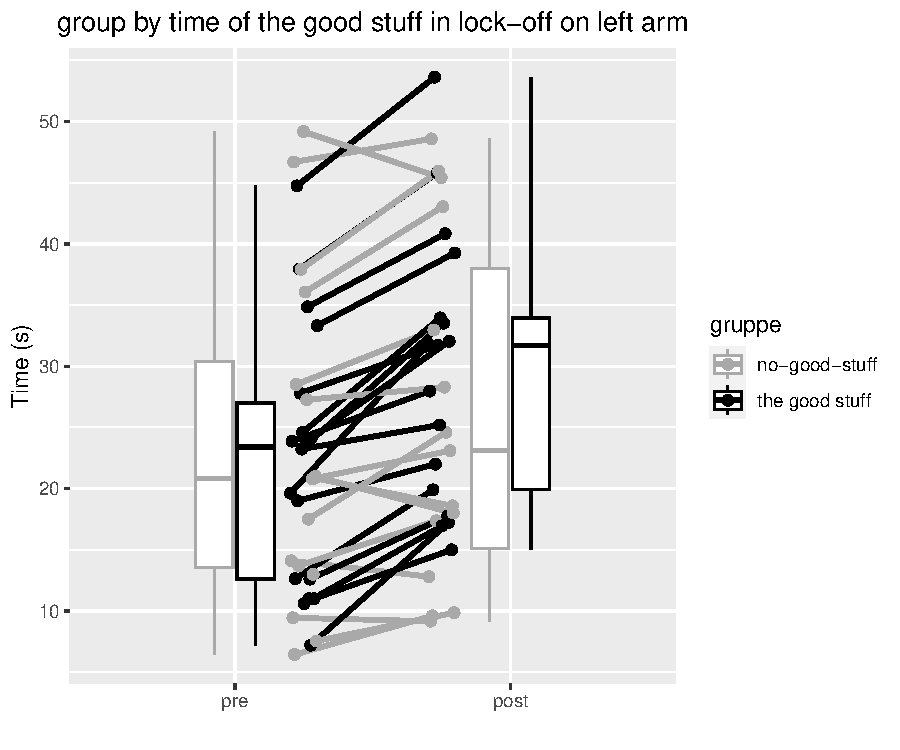
\includegraphics{Data-analysis_files/figure-latex/unnamed-chunk-7-1.pdf}
\caption{This is the figure caption to make the space fit}
\end{figure}

\begin{figure}
\centering
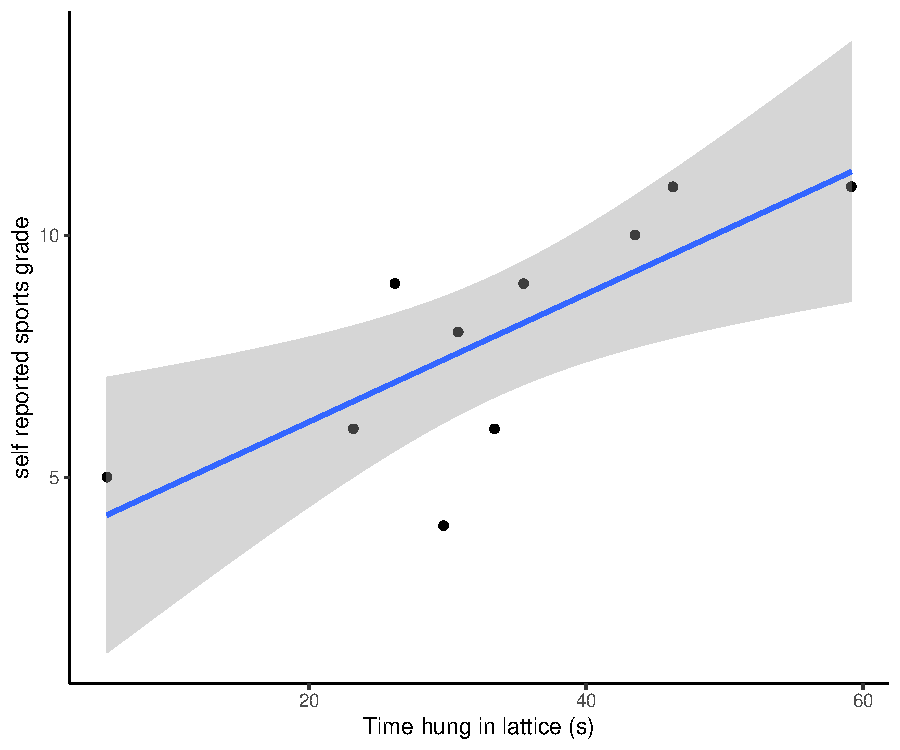
\includegraphics{Data-analysis_files/figure-latex/unnamed-chunk-10-1.pdf}
\caption{This is the figure caption to make the space fit}
\end{figure}

\hypertarget{discussion}{%
\section{Discussion}\label{discussion}}

\hypertarget{appendix}{%
\section{Appendix}\label{appendix}}

\end{document}
